\documentclass[tikz,border=2pt]{standalone}
\usepackage{pgfplots}
\usetikzlibrary{shapes.geometric, intersections}
\pgfplotsset{compat=1.7}

\begin{document}
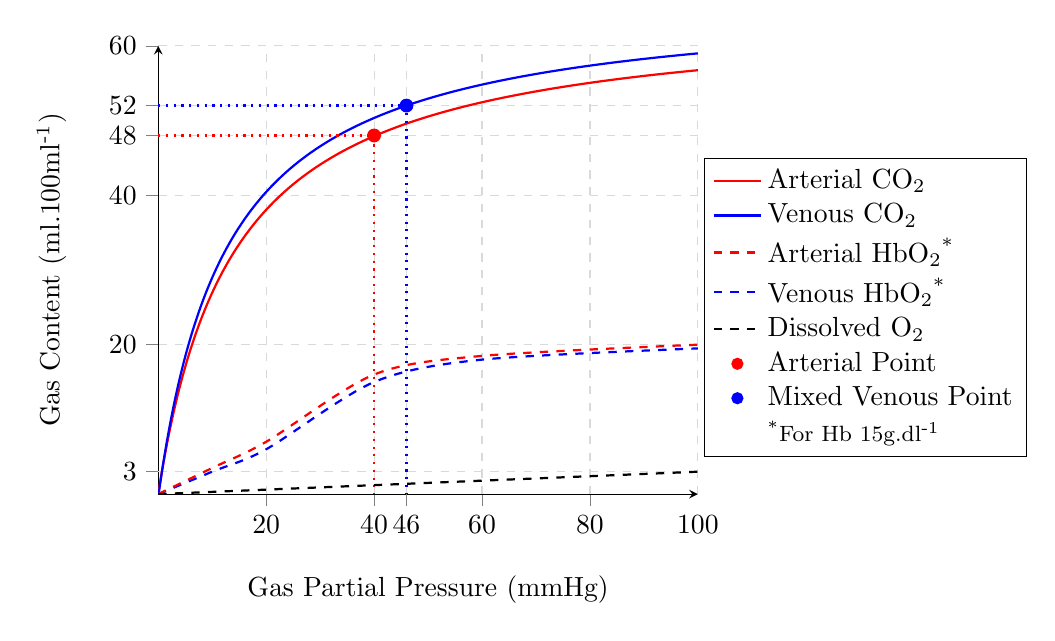
\begin{tikzpicture}

\begin{axis}[
axis lines=middle,
ymin = 0,
ymax = 60,
xmin = 0,
xmax = 100,
grid = major,
grid style={dashed, gray!30},
extra y ticks={3,48,52},
extra x ticks={46},
ylabel near ticks,
xlabel near ticks,
xlabel= Gas Partial Pressure (mmHg),
ylabel= Gas Content (ml.100ml\textsuperscript{-1}),
tick align=outside,
enlargelimits=false,
legend entries={Arterial CO\textsubscript{2},Venous CO\textsubscript{2}, Arterial HbO\textsubscript{2}\textsuperscript{*}, Venous HbO\textsubscript{2}\textsuperscript{*}, Dissolved O\textsubscript{2}, Arterial Point,Mixed Venous Point,\footnotesize{\textsuperscript{*}For Hb 15g.dl\textsuperscript{-1}}},
legend style={name=leg, cells={align=left}, at={(axis cs: 161,45)}},
legend cell align={left}]

\addplot[domain=0:100, red, thick,samples=500] {(64.67682*x)/(13.99809 + x)};
\addplot[domain=0:100, blue, thick,samples=500] {(66.99998*x)/(12.81369 + x) - 0.403};
\draw[blue,thick,dotted] (axis cs: 0,52) -- (axis cs: 46, 52) node[circle,fill=blue,inner sep=0pt,minimum size=5pt]{} -- (axis cs: 46,0);
\draw[red,thick,dotted] (axis cs: 0,48) -- (axis cs: 40,48) node[circle,fill=red,inner sep=0pt,minimum size=5pt]{} -- (axis cs: 40,0);

\draw[blue, thick, dashed] plot[smooth,tension=0.5] coordinates { (axis cs: 0,0)  (axis cs: 10,3) (axis cs: 20,6) (axis cs: 40,15) (axis cs: 60,18) (axis cs: 100,19.5)};
\draw[red, thick, dashed] plot[smooth,tension=0.5] coordinates {(axis cs: 0,0)  (axis cs: 10,3.5) (axis cs: 20,7) (axis cs: 40,16) (axis cs: 60,18.5) (axis cs: 100,20)};
\draw[black, thick, dashed] (axis cs: 0,0) -- (axis cs: 100,3);

\addlegendimage{red, thick, dashed};
\addlegendimage{blue, thick, dashed};
\addlegendimage{black, dashed, thick};
\addlegendimage{only marks,red, mark=*};
\addlegendimage{only marks,blue,mark=*};
\addlegendimage{white, thick};

\end{axis}
\end{tikzpicture} 

\end{document}